% Lab Report 2 (week 2, v0) -- AM/ME/CE 295, Shear-Aware Agentic Grasping.
% Structure follows docs/Lab_Report_Template_Agent_Project.pdf (sections A-E + AI usage disclosure).
% Build: pdflatex LR2_week2_v0.tex (twice). Figures: python make_figures.py (fig/fig_verify.pdf, fig/fig_ablation.pdf).
\documentclass[10pt]{article}
\usepackage[letterpaper,margin=0.72in,top=0.6in,bottom=0.65in]{geometry}
\usepackage{mathptmx}
\usepackage[T1]{fontenc}
\usepackage{microtype,graphicx,booktabs,tabularx,enumitem,amsmath,array,xcolor,tikz}
\usepackage[font=footnotesize,labelfont=bf,skip=4pt]{caption}
\usepackage{placeins}
\usepackage[hidelinks]{hyperref}
\usetikzlibrary{arrows.meta,positioning,fit,backgrounds,calc}

\definecolor{tplorange}{HTML}{E2690C}
\definecolor{tplband}{HTML}{FCE8D8}
\definecolor{tplrow}{HTML}{F1F2F4}
\definecolor{ink2}{HTML}{52514E}
\definecolor{cA}{HTML}{2A78D6}  % agent
\definecolor{cB}{HTML}{EB6834}  % monitor
\definecolor{cC}{HTML}{1BAF7A}  % low level
\definecolor{cD}{HTML}{6B6A66}  % plant

\setlength{\parindent}{0pt}
\setlength{\parskip}{3pt}
\setlist{nosep,leftmargin=1.2em}
\newcommand{\code}[1]{\texttt{\small #1}}
\newcolumntype{L}[1]{>{\raggedright\arraybackslash}p{#1}}

% template-style headers: orange letter on a light-orange band, numbered questions on a grey band
\newcommand{\tplsec}[3]{\par\vspace{7pt}\noindent\colorbox{tplband}{\parbox{\dimexpr\linewidth-2\fboxsep}{%
  \vspace{2pt}{\color{tplorange}\large\bfseries #1}\hspace{0.5em}{\large\bfseries #2}%
  \ifx&#3&\else\\[-1pt]{\small\itshape\color{ink2}#3}\fi\vspace{2pt}}}\par\vspace{3pt}}
\newcommand{\tplq}[2]{\par\vspace{3pt}\noindent\colorbox{tplrow}{\parbox{\dimexpr\linewidth-2\fboxsep}{%
  {\color{tplorange}\bfseries #1}\hspace{0.45em}\textbf{#2}}}\par\vspace{1pt}}

\begin{document}

%------------------------------------------------------------------------------------------- title block
{\Large\bfseries AM/ME/CE 295 $\cdot$ Lab Report 2} \hfill {\small\color{ink2}Week 2 report, v0 $\cdot$ October 31, 2026}\\[3pt]
{\large\bfseries Shear-Aware Agentic Grasping: a thin tactile skin, a verified simulator, and when the agent should take
over}\\[4pt]
\textbf{Team:} Dohyun (\href{https://github.com/DHLeexpress}{@DHLeexpress}) and Jihoon (\href{https://github.com/jhahn2}{@jhahn2})
\quad \textbf{GitHub:} \href{https://github.com/DHLeexpress/ME295}{github.com/DHLeexpress/ME295}

\begin{figure}[h]
\centering
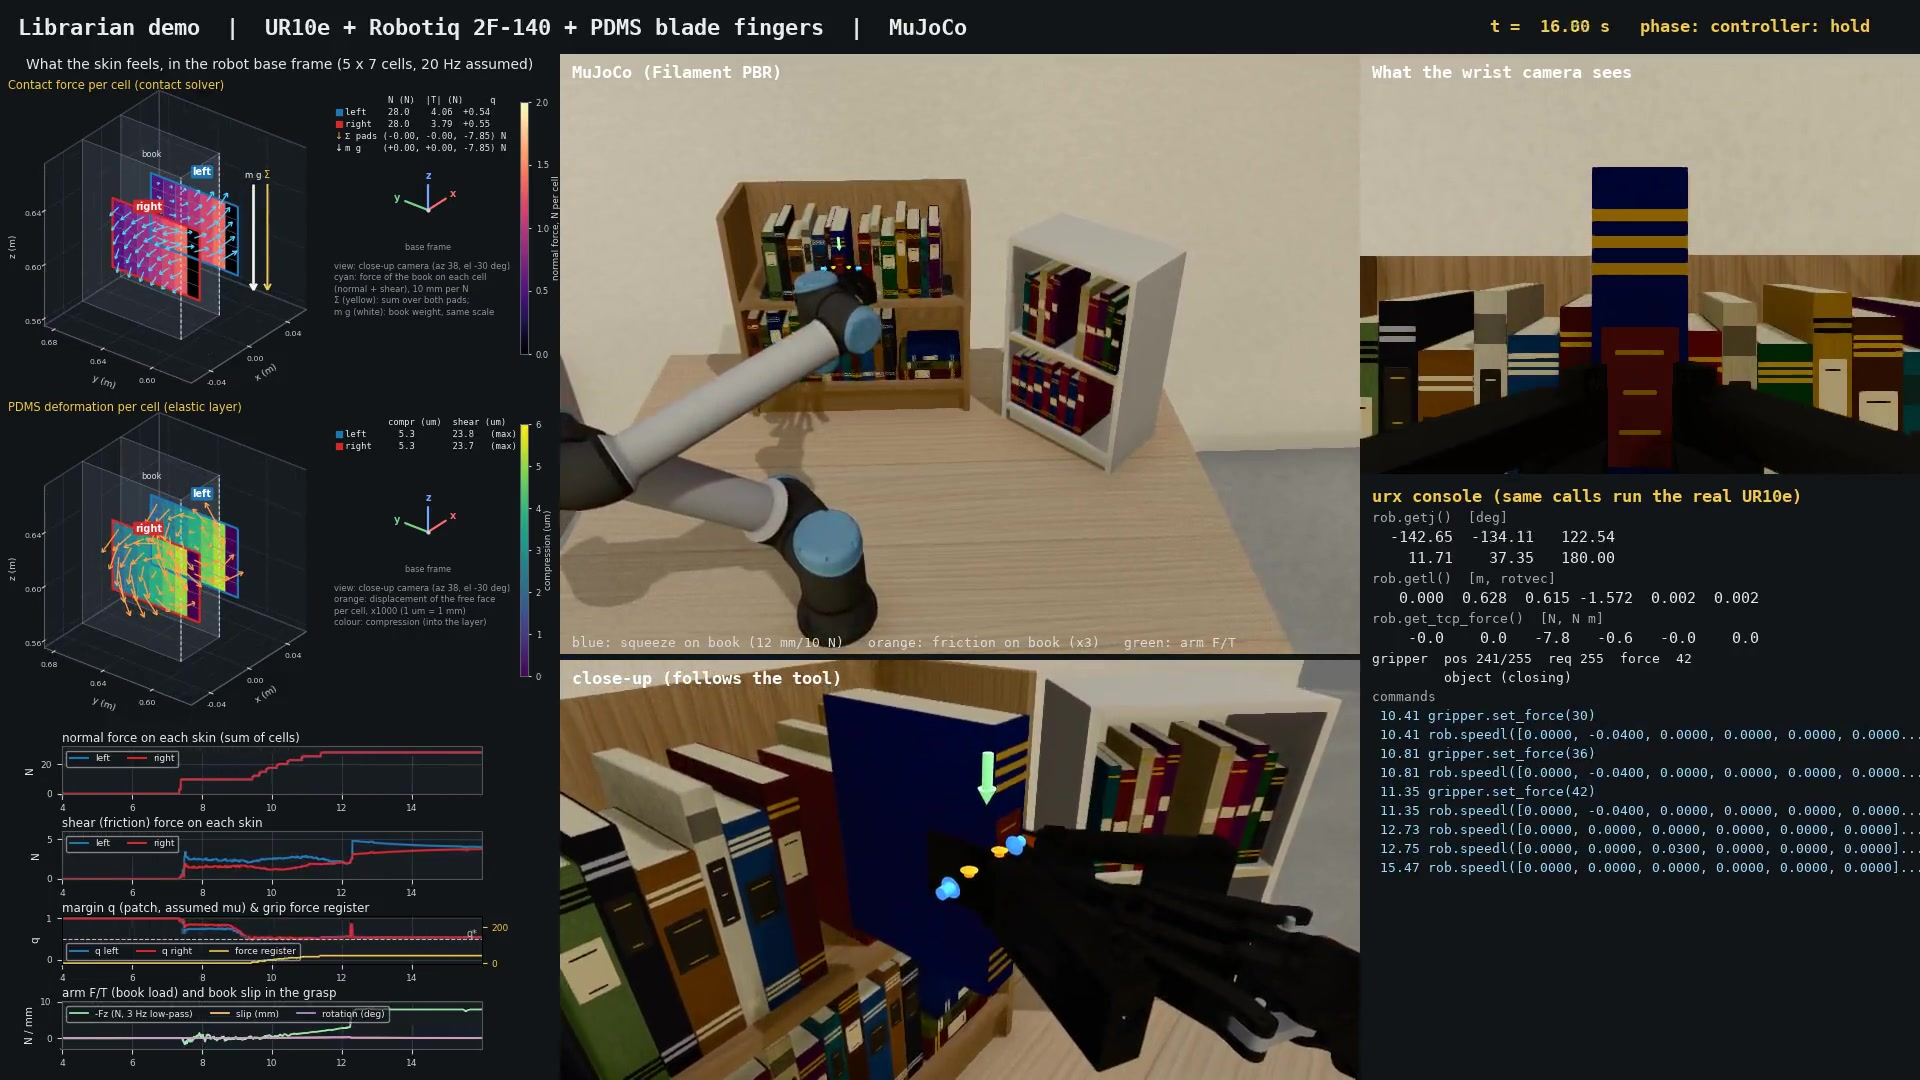
\includegraphics[width=\linewidth]{fig/fig_demo_frame.jpg}
\caption{The simulated system holding a book it has just pulled out of shelf A ($t=16$\,s of the demo video). Left: what
the two PDMS skins feel, drawn in the robot base frame (per-cell contact force, the book's weight $m\mathbf g$ against
the summed pad forces, per-cell deformation $\times1000$) and the controller's time series. Centre: MuJoCo views. Right:
wrist camera and the python-urx console; the same calls drive the real UR10e.}
\label{fig:demo}
\end{figure}
\vspace{-6pt}

%------------------------------------------------------------------------------------------- A
\tplsec{A}{Project description \& goal}{}
\tplq{1}{Problem statement \& goal}
A parallel-jaw gripper knows how far it has closed and roughly how hard it squeezes, but not how close each contact is
to slipping, and inside a packed bookshelf a camera cannot see it either. Jihoon's thin PDMS tactile skin, mounted on
custom blade fingers of a Robotiq 2F-140, measures the contact field that the friction-cone margin needs. We use it at
three levels: (A) a grip controller that squeezes just enough, (B) the task of pulling one book sideways out of a packed
shelf and shelving it elsewhere, and (C) an LLM agent that calls tactile tools to choose and repair contact strategies
when the scripted pipeline fails. The goal is extraction that is more reliable and gentler than fixed-force,
slip-reactive, LLM-prior and vision-only baselines, verified first in a physics-checked simulator and then on the UR10e.

\tplq{2}{Related work}
\textbf{Domain.} Tactile grip control raises force on slip or holds a friction margin
\cite{romano2011,dong2017,dong2019maintaining,su2015force}; friction can be estimated online before gross slip
\cite{khamis2021friction}, and more force does little against rotational slip, which calls for a regrasp
\cite{kolamuri2021rotation}. Book retrieval has used a dexterous finger to tilt a book plus a second arm to grasp it,
without contact sensing \cite{wieczorek2022trixi}, or force-guided search with a two-finger hand \cite{prats2008uji};
tilting and pivoting are planned or executed with force control \cite{hou2019pivot,hou2019hybrid} or learned in
simulation \cite{zhou2022ungraspable}. Contact-rich planning smooths contact models for global planning and local
control \cite{pang2023tro,suh2025ctr,suh2025thesis}, and sampling MPC runs directly on MuJoCo
\cite{howell2022mjpc,li2025judo}. Skins are simulated as local springs or penalties \cite{tacsl2025,elandt2019},
superposed kernels \cite{taxim2021} or volumetric FEM \cite{difftactile2024}; a local (Winkler) layer is only an
approximation \cite{johnson1985,chandler_vella2020}.
\textbf{Agents.} LLMs set grasp physics open-loop from language \cite{xie2024deligrasp}, write robot programs that call
perception and control primitives \cite{liang2023cap}, or plan with keypoint constraints and backtrack on failure
\cite{huang2024rekep}; failures are detected and replanned from execution feedback \cite{guo2024doremi,liu2023reflect},
and hierarchical VLA systems split slow reasoning from fast control \cite{shi2025hirobot,xue2025rdp}.
\textbf{Gap.} Nobody exposes a thin parallel-jaw skin's shear margin to an agent as a tool, on a confined task where
vision is weak; and the agent literature rarely says \emph{when} a planner is needed in a contact-rich task.

%------------------------------------------------------------------------------------------- B
\tplsec{B}{Why an agent}{}
\tplq{1}{Why does this problem need an agent, and not a fixed script, an optimizer, or a single prompt?}
Our scripted pipeline already solves the nominal case (Sec.~C3): gaps wide enough, book mass within the gripper's
force, friction as assumed. The cases it cannot solve are not gain problems but choices between \emph{contact
strategies} (Table~\ref{tab:hl}): a jammed or too-narrow gap needs a different primitive (tilt the book out by its top
edge, search sideways for the gap), a book too heavy for the grip needs a regrasp nearer its centre of mass or a drag
along the board, and an occupied target slot needs a new plan. A \textbf{fixed script} would have to enumerate every
combination of failure and scene in advance; it can only abort today. An \textbf{optimizer} (MPC on the contact
model) handles continuous, local control well \cite{pang2023tro,li2025judo}, but not a discrete, non-local choice of
strategy, nor scene semantics such as which book or which slot. A \textbf{single prompt} cannot close the loop: the
choice depends on what the skin and the guards report \emph{during} the attempt. We therefore keep fast control in
code and give the agent the discrete decisions, called only when a guard fires, with tools that report touch
\cite{liang2023cap,guo2024doremi,huang2024rekep}.

\begin{table}[h]\centering\footnotesize
\caption{When the scripted pipeline needs the agent (from our verified literature survey; boundaries still to be
measured in simulation). LL: the low level suffices; HL: high-level agent.}
\label{tab:hl}\setlength{\tabcolsep}{3.5pt}
\begin{tabularx}{\linewidth}{@{}L{3.3cm}L{4.6cm}cX@{}}\toprule
case & signal in our system & level & strategy from the literature\\\midrule
nominal (today's demo) & guards silent, margin $q\ge q^\star=0.5$ & -- & scripted phases (Sec.~C3)\\
heavier book, within 125\,N & force register rises, $q$ recovers & LL & raise grip on slip \cite{romano2011}; ours 15--83\,N\\
too heavy, or twists & abort: $q<0.2$ at full force for 1\,s & HL & regrasp nearer the CoM \cite{kolamuri2021rotation}; pull, regrasp, pull \cite{prats2008uji}; pivot \cite{hou2019pivot}; choose by force feasibility \cite{holladay2021}\\
gap too narrow & insert guard: wrist $|F|>15$\,N early & HL & sideways search \cite{prats2008uji}; tilt by the top edge \cite{prats2008riai,wieczorek2022trixi}; hybrid force-velocity tilt \cite{hou2019hybrid}\\
friction overestimated & none: $q$ stays high (blind spot) & LL first & slip detection, online $\mu$ \cite{su2015force,khamis2021friction,dong2019maintaining}\\
jam, or slot B blocked & pause/abort in the pull; shelve guard 10\,N & HL & replan on failure \cite{guo2024doremi,liu2023reflect}\\\bottomrule
\end{tabularx}
\end{table}

%------------------------------------------------------------------------------------------- C
\tplsec{C}{Agent design}{What the system is made of, and why each part is there.}
\tplq{1}{Agent design: agents, tools, data and information flow}

\begin{figure}[h]
\centering
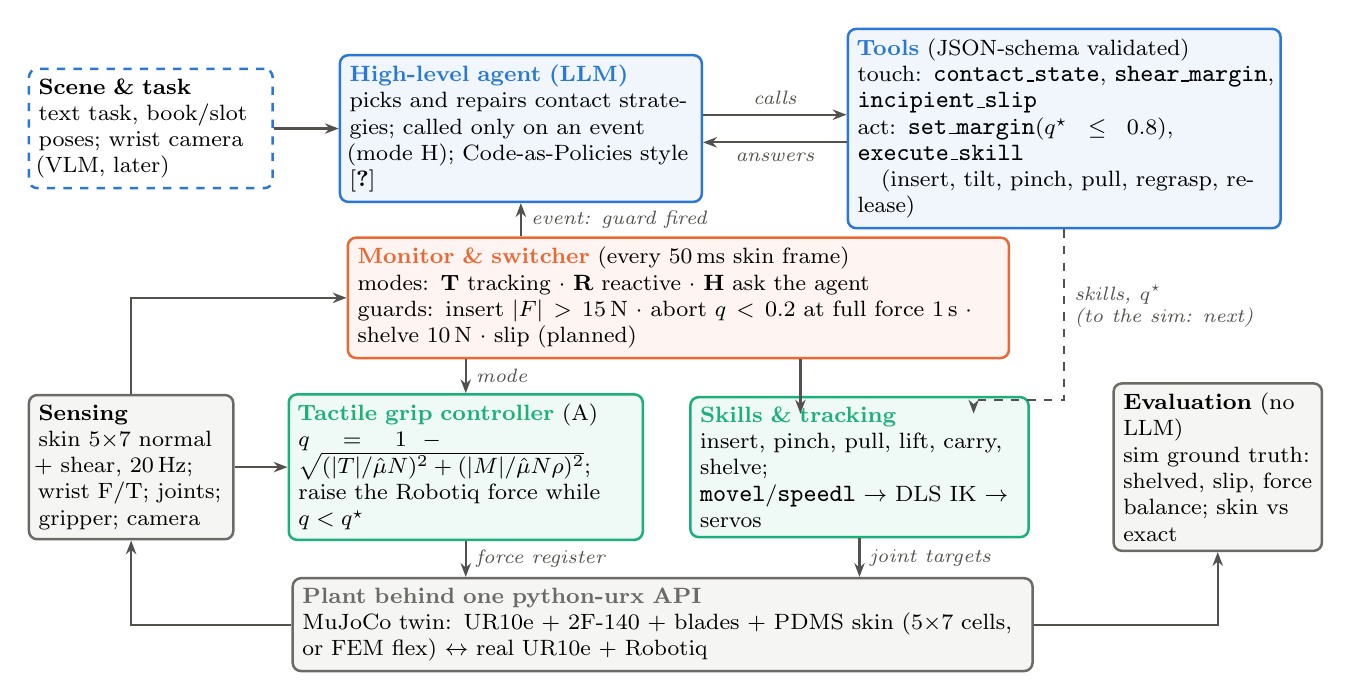
\begin{tikzpicture}[font=\footnotesize, >={Stealth[length=5pt]},
  box/.style={draw=#1, line width=0.9pt, rounded corners=3pt, fill=#1!7, align=left, inner sep=3.5pt},
  plan/.style={draw=#1, line width=0.9pt, rounded corners=3pt, fill=white, align=left, inner sep=3.5pt, dashed},
  lab/.style={font=\scriptsize\itshape, text=ink2},
  arr/.style={->, line width=0.8pt, draw=ink2}]
% row 1: scene, agent, tools
\node[plan=cA, text width=2.85cm] (scene) at (1.75,0) {\textbf{Scene \& task}\\ text task, book/slot poses;
  wrist camera (VLM, later)};
\node[box=cA, text width=4.35cm] (agent) at (6.45,0) {\textbf{\color{cA}High-level agent (LLM)}\\ picks and repairs contact
  strategies; called only on an event (mode H); Code-as-Policies style \cite{liang2023cap}};
\node[box=cA, text width=5.25cm] (tools) at (13.35,0) {\textbf{\color{cA}Tools} (JSON-schema validated)\\
  touch: \code{contact\_state}, \code{shear\_margin}, \code{incipient\_slip}\\ act: \code{set\_margin}$(q^\star\le0.8)$,
  \code{execute\_skill}\\ \quad(insert, tilt, pinch, pull, regrasp, release)};
% row 2: monitor
\node[box=cB, text width=8.15cm] (mon) at (8.45,-2.15) {\textbf{\color{cB}Monitor \& switcher} (every 50\,ms skin frame)\\
  modes: \textbf{T} tracking $\cdot$ \textbf{R} reactive $\cdot$ \textbf{H} ask the agent\\ guards: insert $|F|>15$\,N $\cdot$
  abort $q<0.2$ at full force 1\,s $\cdot$ shelve 10\,N $\cdot$ slip (planned)};
% row 3: sensing, controllers, evaluation
\node[box=cD, text width=2.35cm] (sense) at (1.5,-4.3) {\textbf{Sensing}\\ skin 5$\times$7 normal + shear, 20\,Hz;
  wrist F/T; joints; gripper; camera};
\node[box=cC, text width=4.25cm] (grip) at (5.75,-4.3) {\textbf{\color{cC}Tactile grip controller} (A)\\
  $q=1-\sqrt{(|T|/\hat\mu N)^2+(|M|/\hat\mu N\rho)^2}$;\\ raise the Robotiq force while $q<q^\star$};
\node[box=cC, text width=4.05cm] (track) at (10.75,-4.3) {\textbf{\color{cC}Skills \& tracking}\\ insert, pinch, pull, lift,
  carry, shelve;\\ \code{movel}/\code{speedl} $\to$ DLS IK $\to$ servos};
\node[box=cD, text width=2.4cm] (eval) at (15.3,-4.3) {\textbf{Evaluation} (no LLM)\\ sim ground truth: shelved, slip,
  force balance; skin vs exact};
% row 4: plant
\node[box=cD, text width=9.15cm] (plant) at (8.25,-6.3) {\textbf{\color{cD}Plant behind one python-urx API}\\ MuJoCo twin:
  UR10e + 2F-140 + blades + PDMS skin (5$\times$7 cells, or FEM flex) $\leftrightarrow$ real UR10e + Robotiq};
% arrows
\draw[arr] (scene.east) -- (agent.west);
\draw[arr] ([yshift=5pt]agent.east) -- node[lab, above]{calls} ([yshift=5pt]tools.west);
\draw[arr] ([yshift=-5pt]tools.west) -- node[lab, below]{answers} ([yshift=-5pt]agent.east);
\draw[arr] (mon.north -| agent.south) -- node[lab, right]{event: guard fired} (agent.south);
\draw[arr, dashed] (tools.south) -- node[lab, right, pos=0.45, align=left]{skills, $q^\star$\\(to the sim: next)}
  (tools.south |- 0,-3.45) -- (12.2,-3.45) -- (12.2,-3.62);
\draw[arr] (mon.south -| grip.north) -- node[lab, right]{mode} (grip.north);
\draw[arr] (mon.south -| 10.0,0) -- (10.0,-3.62);
\draw[arr] (grip.south) -- node[lab, right]{force register} (grip.south |- plant.north);
\draw[arr] (track.south) -- node[lab, right]{joint targets} (track.south |- plant.north);
\draw[arr] (plant.west) -| (sense.south);
\draw[arr] (sense.north) |- (mon.west);
\draw[arr] (sense.east) -- (grip.west);
\draw[arr] (plant.east) -| (eval.south);
\end{tikzpicture}
\caption{Agent design. Solid: implemented (tools, validator and LLM loop run offline against a mock robot; guards,
controllers, skills and the twin run in MuJoCo). Dashed: next steps (the agent's skills wired to the simulator, the
slip detector, vision). The agent never commands forces: it chooses skills and the margin $q^\star$, and the code below
executes them.}
\label{fig:arch}
\end{figure}

\begin{minipage}{\linewidth}
\tplq{2}{Why is each role and tool needed, and what stops working without it?}
{\footnotesize\setlength{\tabcolsep}{4pt}
\begin{tabularx}{\linewidth}{@{}L{3.1cm}L{5.5cm}X@{}}\toprule
part & what it does & if removed\\\midrule
PDMS skin + readout & per-cell normal/shear force and deformation, 20\,Hz & no margin: the grip must be fixed; a fixed force is either too weak for heavy books or always maximal (Fig.~\ref{fig:abl})\\
tactile grip controller & squeezes just enough: holds $q\ge q^\star$ & 4/4 books still shelve at 121\,N, but with 1.5--8$\times$ the squeeze (Fig.~\ref{fig:abl})\\
monitor and guards & detect insert, abort and shelve failures; decide T/R/H & the agent is never called (every failure ends in an abort), or is called every step (seconds of LLM latency inside a 50\,ms loop)\\
high-level agent & picks the next contact strategy and its parameters after an event & the system can only put the book back; no recovery from a narrow gap, heavy book or blocked slot\\
tool schemas + validator & typed, bounded actions ($q^\star\le0.8$, skill enum, no free forces) & a malformed or unsafe model output could reach the robot\\
verified twin (python-urx API) & the same task script runs in MuJoCo and on the UR10e; ground truth for every run & no safe place to test recovery; no way to tell a skin artifact from physics (Sec.~C3)\\\bottomrule
\end{tabularx}}
\end{minipage}

\tplq{3}{Current working modules and demonstration}
\textbf{(i) Simulator and scripted task (B, A).} A MuJoCo 3.17 model of the UR10e, the 2F-140 and our blade
(\code{gripper\_dohyun\_v1}, bolted through the fingertip's lug hole) carries the 51$\times$71$\times$1.5\,mm PDMS
layer (0.5\,mm proud of the blade; linear elastic, placeholders $E=1$\,MPa, $\nu=0.45$, no damping). The librarian task
approaches shelf A horizontally, slides both blades into the $\sim$10\,mm gaps beside a 40\,mm book, squeezes it with
the tactile controller, pulls it out 21\,cm, lifts it, carries it by trajectory tracking and shelves it in a 70\,mm
slot of shelf B (Fig.~\ref{fig:demo}). It succeeds with a 1.8\,mm centre error (37\,s simulated, 1\,min 49\,s wall).
The task uses only python-urx calls, so it is written to run unchanged on the UR10e; hardware runs are planned for
LR3. A 3D skin panel in the robot base frame was checked against MuJoCo: while the book hangs, the summed pad forces
equal $-m\mathbf g$ within 0.19\,N.

\textbf{(ii) Does the skin help? (Fig.~\ref{fig:abl}).} In 40 simulated runs (5 grip strategies $\times$ 4 book masses
$\times$ 2 true friction coefficients; the skin assumes $\hat\mu=1$) the skin controller shelved every book when its
friction estimate was right, squeezing 15--83\,N per blade instead of a fixed 121\,N; fixed forces below 70\,N dropped
or misplaced the heavy books. When the true friction was half the estimate, the skin failed every time: the force-ratio
margin cannot see slip when $\mu$ is overestimated. This blind spot is the first thing the agent layer and a slip
detector must handle (Table~\ref{tab:hl}).

\begin{figure}[!b]
\centering
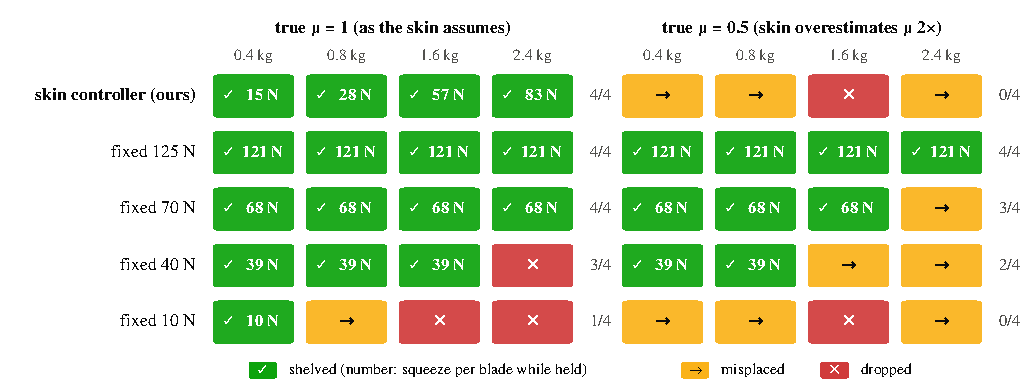
\includegraphics[width=0.98\linewidth]{fig/fig_ablation.pdf}
\caption{Grip ablation in the simulated librarian task (\code{results/ablation\_rev}). Each cell is one run; the number
is the squeeze per blade while the book is held. Right of each group: books shelved out of four.}
\label{fig:abl}
\end{figure}

\textbf{(iii) Is the simulated skin trustworthy? (Fig.~\ref{fig:verify}).} We verified MuJoCo's skin models against
ground truth computed without MuJoCo: an exact integral-transform solution of a layer bonded to a rigid base, with a
boundary-element contact solve, and a converged quadratic finite-element model of the finite pad (the two agree to
0.12\%). Four findings shape the design. (a) MuJoCo's tetrahedral flex uses twice the Lam\'e $\lambda$
(uniaxial strain 1.82$\times$ too stiff, shear exact); a two-line input remap fixes it, and a second MuJoCo defect
(the per-island solver drops the stiffness of a flex pinned to a moving finger) made it diverge on the robot until
islands were disabled. (b) Refining the flex through its 1.5\,mm thickness makes the contact spring softer, so the
reading gets \emph{worse} beyond two elements: overmeshing. (c) The fast 5$\times$7 cell (Winkler) model is within
7\% for a whole-face load at the placeholder $\nu=0.45$, but off by 2.5--30$\times$ for a taxel-sized load at real
PDMS's $\nu\ge0.49$. (d) With the flex on the robot, the full task ran but the book rotated 31\textdegree{} when it left
the shelf: a grasped box resists only about half the exact twist on the flex, and refining the mesh does not help.
The demo therefore runs on the cells, and the flex serves fixed-rig sensor studies. Full study:
\code{docs/report\_flex/flex\_study.pdf}.

\begin{figure}[!t]
\centering
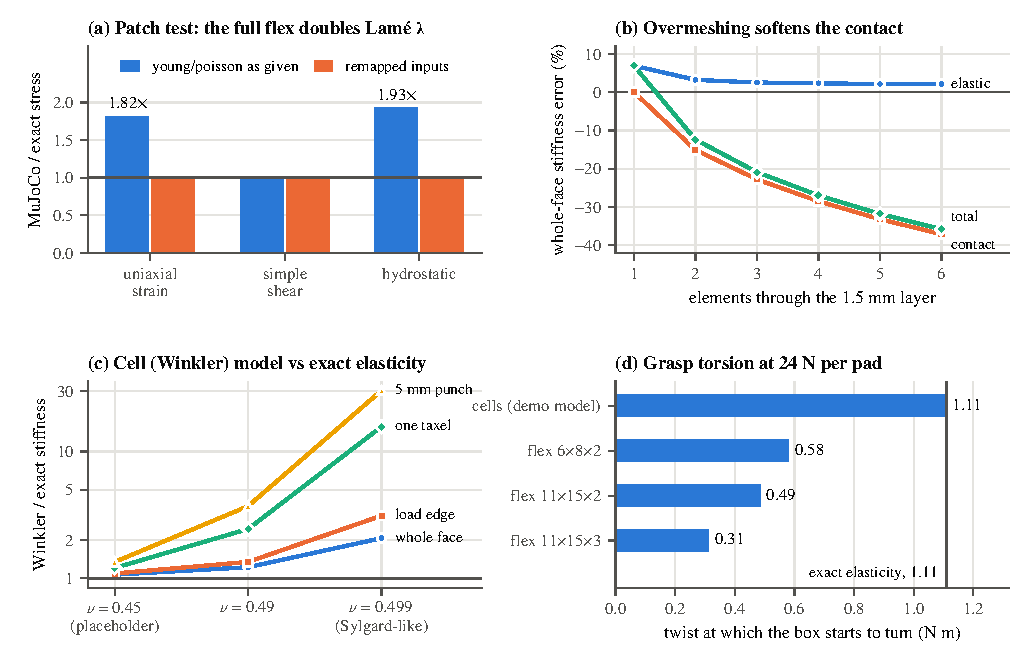
\includegraphics[width=0.98\linewidth]{fig/fig_verify.pdf}
\caption{Verifying the simulated skin against exact solutions. (a) Patch test with exact homogeneous strains: MuJoCo's
full flex vs exact elasticity, before and after the input remap. (b) Whole-face stiffness error against the number of
elements through the layer (20$\times$28 cells): the elastic operator converges, the contact spring softens.
(c) Stiffness of the 5$\times$7 cell model divided by the exact stiffness for four loads. (d) Twist that starts a grasped
box turning at 24\,N per pad: the cells match the exact value, every flex mesh resists about half of it or less.}
\label{fig:verify}
\end{figure}

\textbf{(iv) Agent layer (C).} The tactile tool schemas, the validator, a dependency-free LLM client (Anthropic or
OpenAI-compatible, timeouts, capped retries, token and turn limits) and the tool-use loop run offline with a scripted
mock LLM and a mock gripper (CI runs one episode). The live-model check is still pending an API key, and the tools'
backend is not yet the simulator: wiring \code{execute\_skill} and the margin tools to the MuJoCo skills is the next
step (E1). The hardware track (skin calibration, two-sided acquisition, Robotiq force re-command latency) carries over
from LR1; its status will be updated in v1.

%------------------------------------------------------------------------------------------- D
\FloatBarrier
\tplsec{D}{Evaluation}{How we will know the agent is right, and what it must beat.}
\tplq{1}{What check that does not rely on the LLM tells us the output is right, and what counts as success?}
Every episode is scored from simulator state (later, from the wrist F/T and an external camera), never by the LLM:
\begin{itemize}
\item \textbf{Task:} the book is shelved if its centre lies within 15\,mm horizontally and 8\,mm vertically of the slot
target, with tilt and yaw below 5\textdegree; it is \emph{dropped}, \emph{misplaced} or \emph{put back} otherwise.
\item \textbf{Gentleness and disturbance:} peak and mean squeeze per blade, book slip and rotation in the grasp,
neighbouring-book displacement.
\item \textbf{Physics sanity:} Newton's law on the book closes (3\,mN with the Newton solver; 10\,N with the default CG
cap, which is why we switched); skin models stay within the verified error bounds of Sec.~C3.
\item \textbf{Agent:} recovery rate (failed attempts the agent turns into a shelved book), number of LLM calls and
planner latency; no invalid tool call reaches the robot.
\end{itemize}
\textbf{Success} for LR4: on a randomized scenario set (book mass 0.4--2.4\,kg, friction 0.5--1, gap width, book
position, blocked slot), the agent shelves at least as many books as the best baseline on the nominal cases and
strictly more on the perturbed ones, at lower mean squeeze than a high fixed force.

\tplq{2}{What simpler baseline, with the same tools and no agent, must the agent beat?}
The \textbf{scripted pipeline}: the same skills, tactile controller and guards, with a fixed recovery rule (abort and
put the book back, or one scripted retry). It is today's demo and already beats fixed forces on gentleness
(Fig.~\ref{fig:abl}). The agent must beat it on the perturbed scenarios without losing nominal success or time. We also
keep the proposal's baselines: fixed force (B0), slip-reactive regrasp (B2, \cite{dong2017}), an LLM-prior force with
no touch (B3, \cite{xie2024deligrasp}), scripted tilt-grasp-pull (B4, \cite{wieczorek2022trixi}) and the same agent with
vision-only tools (B5).

%------------------------------------------------------------------------------------------- E
\tplsec{E}{Plan and risks}{What we will build by when, and what could go wrong.}
\tplq{1}{What will work by Lab Report 3 (Nov 15), and by Lab Report 4 (Nov 29)?}
{\footnotesize\setlength{\tabcolsep}{4pt}
\begin{tabularx}{\linewidth}{@{}L{1.55cm}XL{2.2cm}@{}}\toprule
by & deliverable & owner\\\midrule
LR3, Nov 15 & agent tools wired to the MuJoCo skills; monitor with the secure-grasp predicate and T/R/H switching;
scenario sweeps (mass, friction, gap width) that map where the scripted pipeline fails; a slip detector or online
$\hat\mu$ in the low level & Dohyun\\
LR3, Nov 15 & skin calibration (shear $\to$ force against the wrist F/T), Robotiq force re-command latency, one-sided
grip control on the UR10e vs fixed force & Jihoon, Dohyun\\
LR4, Nov 29 & two-sided sensing on the real gripper; agent recovery on hardware for the narrow-gap (top-edge tilt) and
heavy-book (regrasp) cases on a shelf testbed; baselines B0--B5 on the scenario set & both\\\bottomrule
\end{tabularx}}

\tplq{2}{Biggest risk, and the question we most want to discuss}
\textbf{Risk: the skin in simulation is not yet the skin on the robot.} The sensor is not calibrated, and the simulation
showed how much the skin model matters: the cell model is good for whole-face loads but wrong for taxel-scale loads,
the FEM flex has contact artifacts (half the torsional grip, force sensors blind to it), and real PDMS ($\nu\approx0.5$)
widens every gap. An agent tuned on simulated margins could learn the simulator's errors. Mitigation: keep the agent's
decisions discrete and event-driven, calibrate the skin early, and treat thresholds as parameters re-fit on hardware.
\textbf{Question for the TAs:} is a simulation-only evaluation of the agent (with verified physics) acceptable for LR3
while two-sided sensing arrives, and how many randomized trials per scenario would make the comparison convincing?

%------------------------------------------------------------------------------------------- AI disclosure
\par\vspace{6pt}\noindent\colorbox{tplrow}{\parbox{\dimexpr\linewidth-2\fboxsep}{\footnotesize
\textbf{\color{tplorange}AI usage disclosure.} We used Anthropic's Claude (Claude Code with Claude Opus 5.5, including
multi-agent workflows) extensively in this period: to write and debug the simulation and analysis code (MuJoCo model,
controllers, ablation, flex study, figures), to run numerical studies, for literature search with automated citation
checking (every cited source was fetched and checked against the claim it supports; unverifiable ones were dropped),
and to draft this report. Every number comes from a script or run in the repository. The team is responsible for the
content and reviews all AI-generated code and text before submission.}}

%------------------------------------------------------------------------------------------- references
{\footnotesize
\begin{thebibliography}{99}\setlength{\itemsep}{0pt}\setlength{\parskip}{0pt}
\bibitem{romano2011} J.~M.~Romano, K.~Hsiao, G.~Niemeyer, S.~Chitta, K.~J.~Kuchenbecker, ``Human-inspired robotic grasp control with tactile sensing,'' \emph{IEEE Trans. Robotics}, 27(6):1067--1079, 2011.
\bibitem{dong2017} S.~Dong, W.~Yuan, E.~H.~Adelson, ``Improved GelSight tactile sensor for measuring geometry and slip,'' \emph{IROS}, 2017.
\bibitem{dong2019maintaining} S.~Dong, D.~Ma, E.~Donlon, A.~Rodriguez, ``Maintaining grasps within slipping bounds by monitoring incipient slip,'' \emph{ICRA}, pp.~3818--3824, 2019.
\bibitem{su2015force} Z.~Su, K.~Hausman, Y.~Chebotar, A.~Molchanov, G.~E.~Loeb, G.~S.~Sukhatme, S.~Schaal, ``Force estimation and slip detection/classification for grip control using a biomimetic tactile sensor,'' \emph{IEEE-RAS Humanoids}, pp.~297--303, 2015.
\bibitem{khamis2021friction} H.~Khamis, B.~Xia, S.~J.~Redmond, ``Real-time friction estimation for grip force control,'' \emph{ICRA}, pp.~1608--1614, 2021.
\bibitem{kolamuri2021rotation} R.~Kolamuri, Z.~Si, Y.~Zhang, A.~Agarwal, W.~Yuan, ``Improving grasp stability with rotation measurement from tactile sensing,'' \emph{IROS}, pp.~6809--6816, 2021.
\bibitem{wieczorek2022trixi} F.~Wieczorek, S.-C.~Liu, B.~Sygo, M.~Koshil, ``Trixi the librarian,'' arXiv:2210.10110, 2022.
\bibitem{prats2008uji} M.~Prats, E.~Mart\'inez, P.~J.~Sanz, A.~P.~del~Pobil, ``The UJI librarian robot,'' \emph{Intelligent Service Robotics}, 1(4):321--335, 2008.
\bibitem{hou2019pivot} Y.~Hou, Z.~Jia, M.~T.~Mason, ``Reorienting objects in 3D space using pivoting,'' arXiv:1912.02752, 2019.
\bibitem{hou2019hybrid} Y.~Hou, M.~T.~Mason, ``Robust execution of contact-rich motion plans by hybrid force-velocity control,'' \emph{ICRA}, pp.~1933--1939, 2019.
\bibitem{zhou2022ungraspable} W.~Zhou, D.~Held, ``Learning to grasp the ungraspable with emergent extrinsic dexterity,'' \emph{CoRL}, PMLR 205:150--160, 2022.
\bibitem{pang2023tro} T.~Pang, H.~J.~T.~Suh, L.~Yang, R.~Tedrake, ``Global planning for contact-rich manipulation via local smoothing of quasi-dynamic contact models,'' \emph{IEEE Trans. Robotics}, 39(6):4691--4711, 2023.
\bibitem{suh2025ctr} H.~J.~T.~Suh, T.~Pang, T.~Zhao, R.~Tedrake, ``Dexterous contact-rich manipulation via the contact trust region,'' \emph{Int. J. Robotics Research}, 45(9):1418--1454, 2026 (arXiv:2505.02291).
\bibitem{suh2025thesis} H.~J.~T.~Suh, \emph{Leveraging Structure for Efficient and Dexterous Contact-Rich Manipulation}, Ph.D. thesis, MIT EECS, 2025.
\bibitem{howell2022mjpc} T.~Howell, N.~Gileadi, S.~Tunyasuvunakool, K.~Zakka, T.~Erez, Y.~Tassa, ``Predictive sampling: Real-time behaviour synthesis with MuJoCo,'' arXiv:2212.00541, 2022.
\bibitem{li2025judo} A.~H.~Li, B.~Hung, A.~D.~Ames, J.~Wang, S.~Le~Cleac'h, P.~Culbertson, ``Judo: A user-friendly open-source package for sampling-based model predictive control,'' arXiv:2506.17184, 2025; \url{https://github.com/rai-opensource/judo}.
\bibitem{tacsl2025} I.~Akinola, J.~Xu, J.~Carius, D.~Fox, Y.~Narang, ``TacSL: A library for visuotactile sensor simulation and learning,'' \emph{IEEE Trans. Robot.}, 41:2645--2661, 2025.
\bibitem{elandt2019} R.~Elandt, E.~Drumwright, M.~Sherman, A.~Ruina, ``A pressure field model for fast, robust approximation of net contact force and moment between nominally rigid objects,'' \emph{IROS}, pp.~8238--8245, 2019.
\bibitem{taxim2021} Z.~Si, W.~Yuan, ``Taxim: An example-based simulation model for GelSight tactile sensors,'' \emph{IEEE Robot. Autom. Lett.}, 7(2):2361--2368, 2022.
\bibitem{difftactile2024} Z.~Si, G.~Zhang, Q.~Ben, B.~Romero, Z.~Xian, C.~Liu, C.~Gan, ``DiffTactile: A physics-based differentiable tactile simulator for contact-rich robotic manipulation,'' \emph{ICLR}, 2024.
\bibitem{johnson1985} K.~L.~Johnson, \emph{Contact Mechanics}, Cambridge Univ. Press, 1985, \S4.3 and \S5.8.
\bibitem{chandler_vella2020} T.~G.~J.~Chandler, D.~Vella, ``Validity of Winkler's mattress model for thin elastomeric layers: beyond Poisson's ratio,'' \emph{Proc. R. Soc. A}, 476(2242):20200551, 2020.
\bibitem{xie2024deligrasp} W.~Xie, M.~Valentini, J.~Lavering, N.~Correll, ``DeliGrasp: Inferring object properties with LLMs for adaptive grasp policies,'' \emph{CoRL}, 2024.
\bibitem{liang2023cap} J.~Liang, W.~Huang, F.~Xia, P.~Xu, K.~Hausman, B.~Ichter, P.~Florence, A.~Zeng, ``Code as policies: Language model programs for embodied control,'' \emph{ICRA}, pp.~9493--9500, 2023.
\bibitem{huang2024rekep} W.~Huang, C.~Wang, Y.~Li, R.~Zhang, L.~Fei-Fei, ``ReKep: Spatio-temporal reasoning of relational keypoint constraints for robotic manipulation,'' \emph{CoRL}, PMLR 270:4573--4602, 2024.
\bibitem{guo2024doremi} Y.~Guo, Y.-J.~Wang, L.~Zha, J.~Chen, ``DoReMi: Grounding language model by detecting and recovering from plan-execution misalignment,'' \emph{IROS}, pp.~12124--12131, 2024.
\bibitem{liu2023reflect} Z.~Liu, A.~Bahety, S.~Song, ``REFLECT: Summarizing robot experiences for failure explanation and correction,'' \emph{CoRL}, 2023.
\bibitem{shi2025hirobot} L.~X.~Shi, B.~Ichter, M.~Equi, L.~Ke, K.~Pertsch, Q.~Vuong, \emph{et al.}, ``Hi Robot: Open-ended instruction following with hierarchical vision-language-action models,'' \emph{ICML}, PMLR 267:54919--54933, 2025.
\bibitem{xue2025rdp} H.~Xue, J.~Ren, W.~Chen, G.~Zhang, Y.~Fang, G.~Gu, H.~Xu, C.~Lu, ``Reactive diffusion policy: Slow-fast visual-tactile policy learning for contact-rich manipulation,'' \emph{RSS}, 2025.
\bibitem{prats2008riai} M.~Prats, P.~J.~Sanz, E.~Mart\'inez, R.~Mar\'in, A.~P.~del~Pobil, ``Manipulaci\'on aut\'onoma multiprop\'osito en el robot de servicios Jaume-2,'' \emph{RIAI}, 5(2):25--37, 2008.
\bibitem{holladay2021} R.~Holladay, T.~Lozano-P\'erez, A.~Rodriguez, ``Planning for multi-stage forceful manipulation,'' \emph{ICRA}, pp.~6556--6562, 2021.
\end{thebibliography}}

\end{document}
